%%%%%%%%%%%%%%%%%%%%%%%%%%%%%%%%%%%%%%%%%%%%%%%%%%%%%%%%%%%
%%% Umsetzung
%%%%%%%%%%%%%%%%%%%%%%%%%%%%%%%%%%%%%%%%%%%%%%%%%%%%%%%%%%%
\chapter{Die theoretische Ausarbeitung des Angriffs} \label{hdl:theroetical-attack}

In diesem Kapitel wird der \ac{MitM} Angriff theoretisch ausgearbeitet und gezeigt, unter welchen Voraussetzungen er in \ac{GSM} umgesetzt werden kann. Die Schwachstellen im \ac{GSM}-Standard, die den Angriff möglich machen werden dargestellt und die Schritte herausgearbeitet, die notwendig sind um ein ausgehendes Telefonat erfolgreich umzuleiten.

\section{Das Problem von Stromverschlüsselung ohne Integrität} \label{hdl:einleitung_verschlue_ohne_int}

\ac{GSM} verwendet Stromverschlüsselung zum Schutz der vertraulichen Kommunikation und ist damit anfällig für "`Known Plaintext"' Angriffe ohne Kenntnis des kryptografischen Schlüssels. Da die Integrität der übertragenen Nachrichten nicht geschützt, ist kann ein \ac{MitM}-Angreifer bekannte Daten beliebig verändern.

\begin{figure}[H]
	\centering 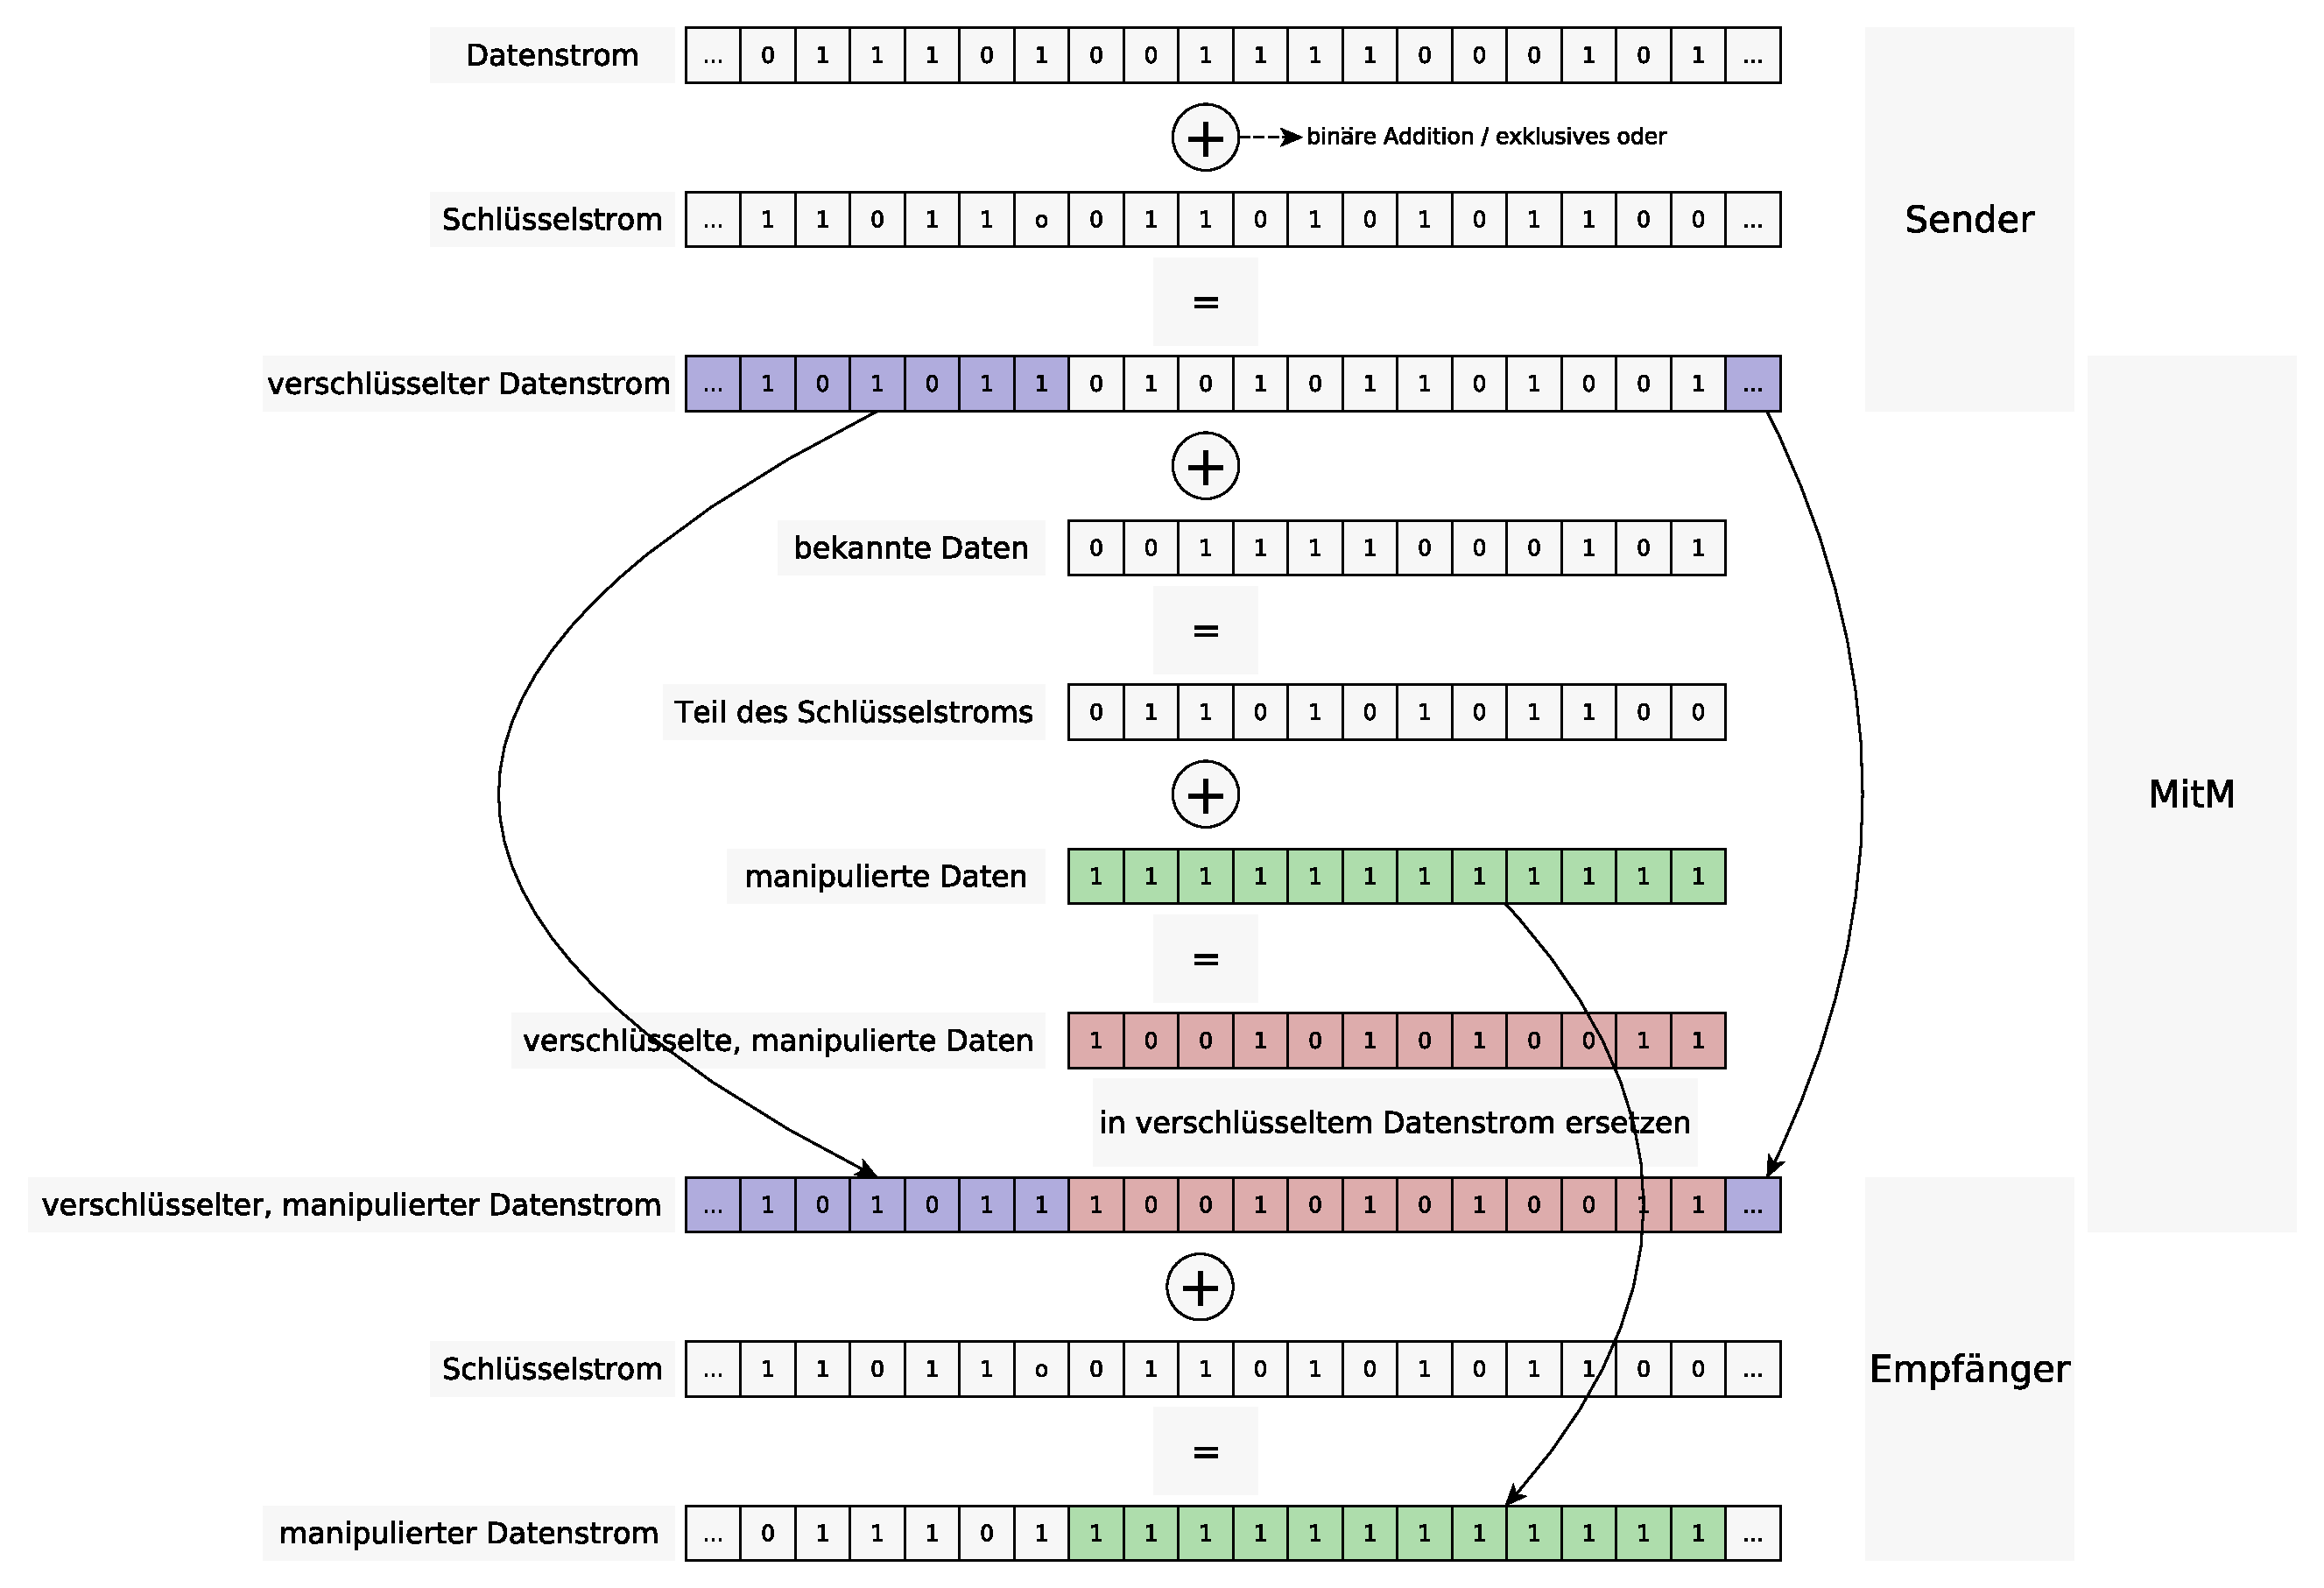
\includegraphics[width=1.0\linewidth]{figures/partially_known_plaintext_manipulation.pdf}
	\caption[Datenmanipulation ohne Kenntnis des kryptografischen Schlüssels]{Datenmanipulation ohne Kenntnis des kryptografischen Schlüssels, erstellt mit yEd} \label{fig:partially-known-plaintext-manipulation}
\end{figure}

\autoref{fig:partially-known-plaintext-manipulation} zeigt an einem Ausschnitt des Datenstroms, wie bekannte Daten trotz Verschlüsselung von einem \ac{MitM} geändert werden können. Da der Chiffrestrom das Ergebnis der \ac{XOR}-Kombination von Datenstrom und Schlüsselstrom ist, kann der Angreifer für bekannte Daten, den verwendeten Schlüsselstrom berechnen. Die Kenntnis des Schlüsselstroms für einen Teil des Datenstroms erlaubt dem Angreifer, diesen Teil beliebig zu manipulieren. Beim Empfänger kommt nach der Entschlüsselung der geänderte Datenstrom heraus. Methoden zum Schutz der Integrität übertragen zusätzlich zu den Nutzdaten in der Regel einen Hashwert, der nur korrekt berechnet werden kann, wenn der vollständige Klartext bekannt ist. Änderungen eines Angreifers, der nur einen Teil der Daten kennt, können also vom Empfänger bemerkt werden. Ohne Methoden zum Schutz der Integrität kann der Empfänger die Manipulation hingegen nicht bemerken.

Die Kenntnis über den mangelnden Schutz von Verschlüsselung ohne Integrität ist weit verbreitet. Dennoch werden darauf basierende Angriffe von verschiedenen Übertragungsprotokollen und deren Spezifikationen ermöglicht. So zeigen \citet{paterson2006cryptography} die Schwachstelle in der \ac{IPSec} Implementierung im Linux Kernel auf. Sie können, wenn \ac{IPSec} ohne Authentifizierung und Integrität konfiguriert ist, die Verschlüsselung von \ac{ESP} Paketen erfolgreich brechen. \citet{degabriele2007attacking} stellen mehrere implementierungsunabhängige Angriffe auf \ac{IPSec} vor und zeigen damit, dass die Schwachstelle in \ac{IPSec} nicht nur im Linux Kernel existiert, sondern in der \ac{IPSec}-Standardisierung. Der für den Standard IEEE 802.11 für Drahtlosnetzwerke spezifizierte Verschlüsselungsalgorithmus \ac{WEP}, leidet an der gleichen Schwachstelle. Er gilt heute offiziell als unsicher, von Herstellern wird generell empfohlen, \ac{WEP} nicht mehr für ihre Geräte zu verwenden. Dennoch besteht nach wie vor die Möglichkeit, die meisten Wlan-Router und andere IEEE 802.11 kompatible Geräte für \ac{WEP} zu konfigurieren. \citet{bittau2006final} stellen einen Fragmentierungsangriff auf \ac{WEP} vor, der wegen seiner kurzen Ausführungszeit, trotz regelmäßiger Erneuerung des Schlüssels funktioniert. Wiederum basiert er auf fehlender Integrität von durch Stromverschlüsselung geschützten Daten. Die Arbeiten weisen alle auf die Gefahren der Nutzung von Verschlüsselung ohne Integrität hin und empfehlen, solche Konfigurationen generell nicht zu unterstützen und zu verwenden.

\section{Die Idee des \acl{MitM} Angriffs auf GSM} \label{hdl:einleitung_mitm-gsm}

\begin{figure}[H]
	\centering 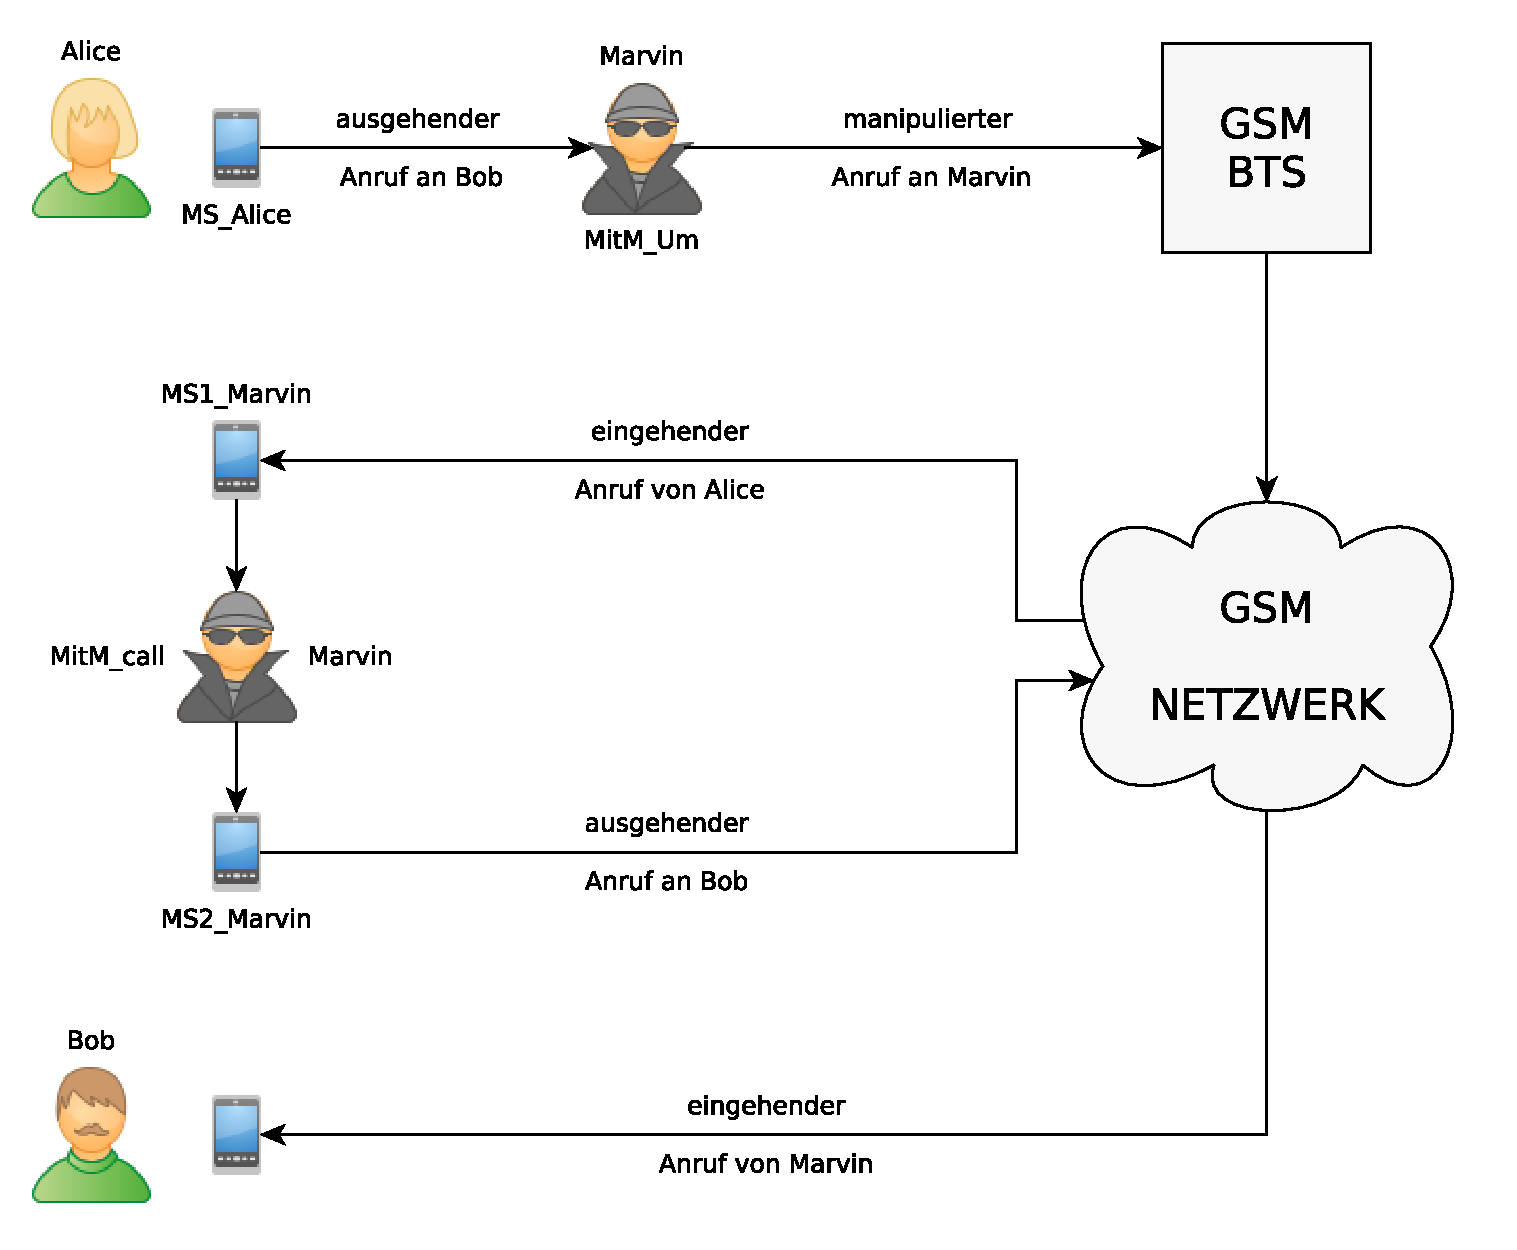
\includegraphics[width=0.9\linewidth]{figures/mitm_attack_overview.pdf}
	\caption[Die Idee des MitM-Angriffs]{Die Idee des \ac{MitM}-Angriffs, erstellt mit yEd} \label{fig:mitm-attack-overview}
\end{figure}

Das Szenario (siehe \autoref{fig:mitm-attack-overview}):

Alice ist mit dem \ac{GSM}-Netz verbunden und möchte Bob anrufen. Der Angreifer Marvin hat ein \ac{MitM}-Gerät ($\ac{MitM}_{Um}$) auf der \ac{Um} Schnittstelle installiert, mit dem er auf physikalischer Ebene Zugriff auf alle ausgetauschten Nachrichten zwischen Alice's Telefon und der \ac{GSM}-\ac{BTS} hat. Die Nachrichten sind kodiert und stromverschlüsselt. Stromverschlüsselung schützt nicht vor Datenmanipulation bei bekanntem Klartext und Bob's Telefonnummer ist Marvin bekannt. Er kann deshalb den Anrufaufbau im $\ac{MitM}_{Um}$ manipulieren und Bob's Telefonnummer austauschen. Da die Integrität der ausgetauschten Nachrichten in \ac{GSM} nicht geschützt ist, können weder Alice noch die \ac{BTS} die Manipulation bemerken. Der manipulierte Anruf wird deshalb vom Netzwerk als gültig erkannt und an Marvin's Mobiltelefon weitergeleitet. Das Netzwerk übernimmt Kodierung und Verschlüsselung des übertragenen Datenstroms, Marvin erhält das Gespräch von Alice im Klartext. Marvin ruft nun Bob an und verknüpft die beiden Anrufe so, dass Bob die Gesprächsdaten von Alice erhält und umgekehrt. Da Marvin Zugriff auf den Klartext beider Datenströme hat, kann er diese aufnehmen und manipulieren. Der dadurch entstandene \ac{MitM}-Angriff ($\ac{MitM}_{call}$) funktioniert unabhängig vom verwendeten Verschlüsselungsverfahren und ist in \autoref{fig:mitm-in-voice-con} dargestellt.

\begin{figure}[H]
	\centering 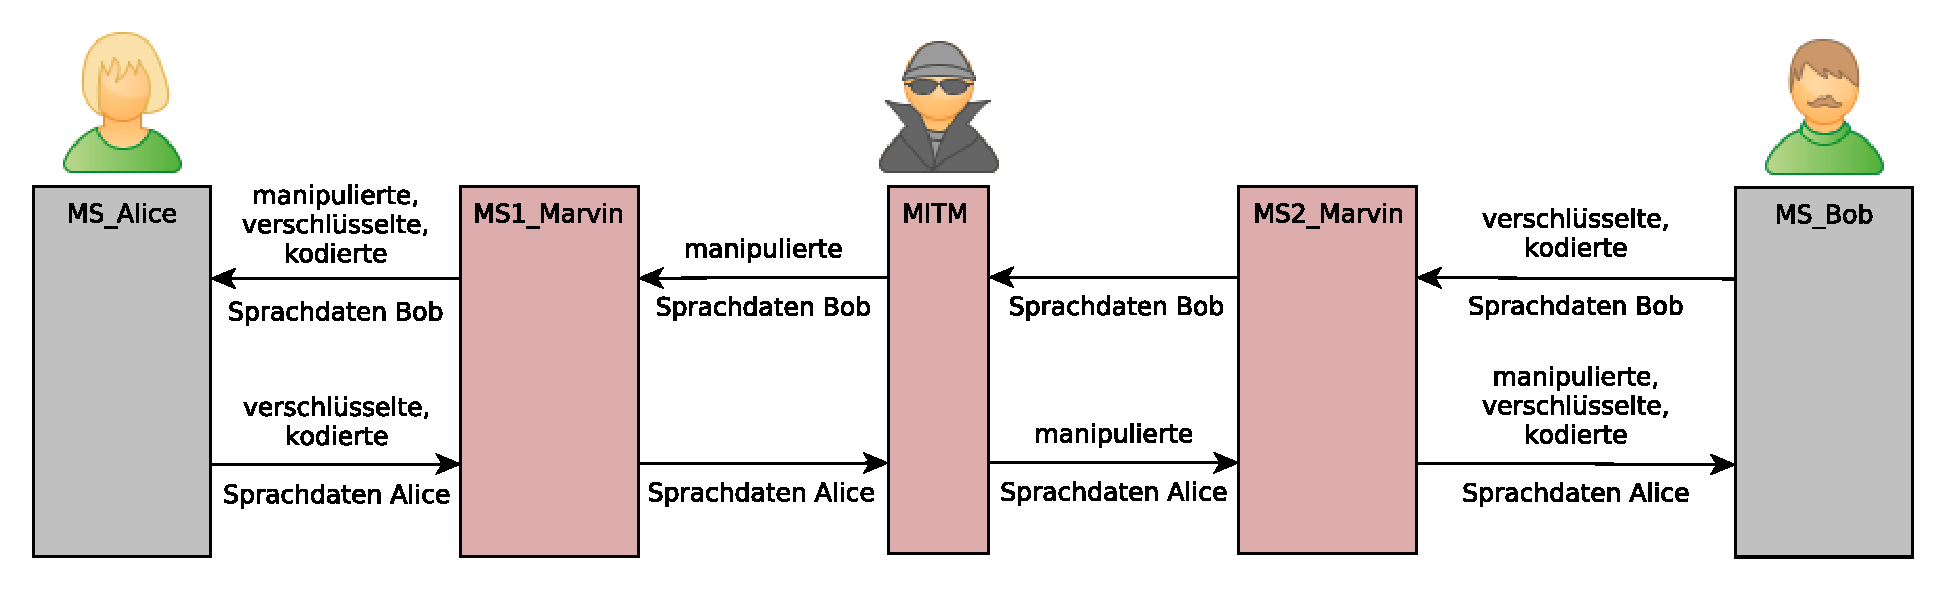
\includegraphics[width=1.0\linewidth]{figures/mitm_in_voice_connection.pdf}
	\caption[Der entwickelte MitM-Angriff auf eine Sprachverbindung]{Der entwickelte \ac{MitM}-Angriff auf eine Sprachverbindung, erstellt mit yEd} \label{fig:mitm-in-voice-con}
\end{figure}

Dass ein \ac{MitM}-Angriff auf dem \ac{Um} möglich ist, haben bereits \citet{barkan2003instant}, \citet{meyer2004man} und \citet{paget2010practical} gezeigt. Für ihre \ac{MitM}-Angriffe verwenden sie eine falsche Basisstation (siehe \autoref{hdl:einleitung_stand-der-technik}). Das \ac{MitM}-Gerät für den vorgestellten Angriff benötigt nur Zugriff auf den verschlüsselten, kodierten Datenverkehr und muss den kryptografischen Schlüssels nicht berechnen. Statt einer falschen Basisstation reicht also ein \ac{MitM}-Gerät auf physikalischer Ebene, mit geringer Rechenleistung aus. Das würde in etwa der Funktionalität eines \ac{GSM}-Repeaters mit zusätzlichen Verarbeitungsroutinen für den Datenstrom entsprechen. Statt Daten nur zu verstärken und weiterzuleiten kann er diese auch analysieren und manipulieren. Die Zeit dafür kann durch die Verzögerung des Datenverkehrs von bis zu $233 \mu s$ gewonnen werden, die die Timing Advance Funktion des \ac{GSM}-Standards erlaubt (siehe \autoref{hdl:ta}). Das \ac{MitM}-Gerät in der Funkschnittstelle, mit Zugriff auf den verschlüsselten und kodierten Datenverkehr, wird in dieser Arbeit vorausgesetzt. Die Möglichkeiten der Nutzung eines modifizierten \ac{GSM}-Repeaters für den \ac{MitM}-Angriff werden nicht untersucht.

\section{Analyse des Nachrichtenflusses auf der Um Schnittstelle beim Anrufaufbau}\label{hdl:call-setup-message-flow-analysis}

Um herauszufinden, welche Nachrichten für den Aufbau einer Telefonverbindung zuständig sind, wird der Nachrichtenfluss auf der Um Schnittstelle analysiert. Folgende Fragen müssen beantwortet werden:
\begin{itemize}
\item Wie wird das Opfer identifiziert?
\item Wie wird die für den Anrufaufbau zuständige "`Setup"' Nachricht im Nachrichtenfluss identifiziert?
\end{itemize}

\autoref{fig:moc-um-1} und Folgende enthalten die zwischen \ac{MS} und \ac{BTS} ausgetauschten Signalisierungsnachrichten. Aktuelle (Stand 2015) Informationen zum untersuchten Nachrichtenfluss finden sich in \citetauthor[Kap. 7.3.2]{3gpp:23.108} und \citetauthor[Abb. A.1]{3gpp:24.007}. Übertragene \ac{RR}-Signalisierungsnachrichten sind in \citetauthor{3gpp:04.18}, \ac{MM} und \ac{CM}-Nachrichten, sowie Service-Requests in \citetauthor{3gpp:24.008} spezifiziert.

\begin{figure}[H]
	\centering \includegraphics[width=1.0\textwidth]{figures/mscgen/gsm_MOC_on_UM01.pdf}
	\caption[Nachrichtenfluss auf der Um-Schnittstelle beim Anrufaufbau, Teil 1]{Nachrichtenfluss auf der \ac{Um}-Schnittstelle beim Anrufaufbau, Teil 1, nach \citepauthor[Kap. 7.3.2]{3gpp:23.108} und \citepauthor[Abb. A.1]{3gpp:24.007}} \label{fig:moc-um-1}
\end{figure}

\begin{description}
\item[1:] Das \ac{MS} beantragt mit dem \texttt{CHANNEL-REQUEST} \citepauthor[Kap. 9.1.8]{3gpp:04.18} einen dedizierten Kanal. Der Request enthält ein Flag, das dem Netzwerk signalisiert, für was der Kanal verwendet werden soll. Bei "`Very Early Assignment"' reserviert das Netzwerk an dieser Stelle einen \ac{TCH}. Das bedeutet, die folgende Signalisierung würde auf dem \ac{FACCH} und nicht wie in der Abbildung auf dem \ac{SDCCH} erfolgen \citepauthor[Kap. 7.3.2]{3gpp:23.108}. Mit dem \texttt{IMMEDIATE-ASSIGNMENT} \citepauthor[Kap. 9.1.18]{3gpp:04.18} erhält das \ac{MS} vom Netzwerk die benötigten Informationen zum reservierten Kanal, was es ihm ermöglicht, auf diesen zu wechseln. Nach dem Wechsel in den "`Dedicated Mode"' beantragt das \ac{MS} auf dem \ac{SDCCH} mit einem \ac{SABM}-Frame den Wechsel vom unacknowledged in den asynchronous balanced \ac{LAPDm}-Modus. Damit initiiert es den Aufbau einer von der Datensicherungsschicht geschützten Verbindung (siehe \autoref{hdl:einfuehrung-gsm_schnittstellen_protokolle-um_interface-layer2}). Das \ac{SABM}-Frame trägt den \texttt{CM-SERVICE-REQUEST} \citepauthor[Kap. 9.2.9]{3gpp:24.008} mit der \ac{IMSI} oder \ac{TMSI} des Netzteilnehmers, dem Typ des angeforderten \ac{CM}-Dienstes und Informationen zu \ac{MS}-seitig unterstützten Verschlüsselungsverfahren mit sich. Der Empfang der \ac{SABM}-Nachricht und der netzwerkseitige Wechsel in den asynchronous balanced Mode, wird durch ein \ac{UA}-Frame mit einer Kopie des erhaltenen Service-Requests bestätigt. Alle weiteren Signalisierungsnachrichten auf dem dedizierten Kanal sind in \ac{I}-Frames verpackt und werden bei erfolgreichem Empfang mit einem \ac{RRm}-Frame bestätigt. Das \ac{RRm}-Frame hat in dem Fall nichts mit \acl{RR} zu tun, sondern ist eine Kontrollnachricht des \ac{LAPDm}-Protokolls. Die Werte der Zähler \ac{N(R)} und \ac{N(S)} für empfangene und gesendetet Nachrichten sind im Flussdiagramm für \ac{I} und \ac{RRm}-Frames dargestellt.
\item[2:] Die Identitätsabfrage des Netzteilnehmers \citep[Kap. 4.3.3]{3gpp:24.008} erfolgt, wenn das Netzwerk die \ac{TMSI} aus dem \texttt{CM-SERVICE-REQUEST} keiner \ac{IMSI} zuweisen kann. Sie sollte nur wenn nötig ausgeführt werden, um die Anonymität der Netzteilnehmer zu schützen, also in der Regel nicht bei jeder Anfrage eines Teilnehmers. Der \texttt{IDENTITY-REQUEST} \citep[Kap. 9.2.10]{3gpp:24.008} enthält den Identitätstyp, der abgefragt wird (\ac{IMSI}, \ac{TMSI}, \ac{IMEI}). Das Netzwerk kann mehr als einen Identity Request schicken um weitere Identitäten anzufordern. Nachdem die \ac{MS} den Request mit einer \texttt{IDENTITY-RESPONSE} \citep[Kap. 9.2.11]{3gpp:24.008} beantwortet und die gewünschte Identität geliefert hat, ist die Routine abgeschlossen.
\item[3:] Wie die Identitätsabfrage erfolgt auch die Authentifizierung nur bei Bedarf. Aus dem \texttt{CM"=SERVICE"=REQUEST} kennt das Netzwerk die aktuellen Sicherheitsparameter des \ac{MS} und kann mit diesen überprüfen, ob ein gültiger Security-Context besteht (siehe \autoref{hdl:keygen}). Existiert kein gültiger Security-Context muss das \ac{AKA} erneut durchgeführt werden, ansonsten kann die Authentifizierung übersprungen werden. Wenn \ac{MS} und \ac{AuC} \ac{UMTS}-fähig sind, wird das \ac{UMTS}-\ac{AKA} ausgeführt (siehe \autoref{hdl:umts-aka}), andernfalls das \ac{GSM}-\ac{AKA} (siehe \autoref{hdl:authentication}). Die ausgetauschten Nachrichten unterscheiden sich dabei nur in der Interpretation des Inhalts von \ac{RES} und \ac{RAND}. Das Netzwerk schickt dem \ac{MS} im \texttt{AUTHENTICATION-REQUEST} \citep[Kap. 9.2.2]{3gpp:24.008}, je nach verwendetem \ac{AKA}, die \ac{GSM} oder \ac{UMTS} Challenge \ac{RAND}. Das \ac{MS} berechnet die Antwort auf die Challenge und schickt sie dem Netzwerk in der \texttt{AUTHENTICATION-RESPONSE} \citep[Kap. 9.2.2]{3gpp:24.008} zurück. Ist die Authentifizierung erfolgreich, kennen beide Seiten auch den synchronen, kryptografischen Schlüssel für das A5 Verschlüsselungsverfahren.
\end{description}

\begin{figure}[H]
	\centering \includegraphics[width=1.0\linewidth]{figures/mscgen/gsm_MOC_on_UM02.pdf}
	\caption[Nachrichtenfluss auf der Um-Schnittstelle beim Anrufaufbau, Teil 2]{Nachrichtenfluss auf der \ac{Um}-Schnittstelle beim Anrufaufbau, Teil 2, nach \citepauthor[Kap. 7.3.2]{3gpp:23.108} und \citepauthor[Abb. A.1]{3gpp:24.007}} \label{fig:moc-um-2}
\end{figure}

\begin{description}
\item[4:] Mit dem \texttt{CIPHERING-MODE-COMMAND} \citep[Kap. 9.1.9]{3gpp:04.18} befiehlt das Netzwerk dem \ac{MS}, von jetzt an die Verschlüsselung des Uplinks zu starten. Sobald die korrekt verschlüsselte \texttt{CIPHERING-MODE-COMPLETE} \citep[Kap. 9.1.10]{3gpp:04.18} Bestätigung des \ac{MS} empfangen wird, beginnt das Netzwerk den Downlink zu verschlüsseln. Der darauf folgende Nachrichtenverkehr auf dem dedizierten Kanal ist bidirektional durch das ausgehandelte, synchrone Verschlüsselungsverfahren (zum Beispiel A5/3) geschützt.
\item[5:] Mit dem Call \texttt{SETUP} \citep[Kap. 9.3.23.2]{3gpp:24.008} wird der Anruf vom \ac{MS} initiiert. Die angerufene Nummer und weitere Informationen zum Anruf werden dem Netzwerk erst in dieser Nachricht mitgeteilt. Um den Anruf umzuleiten, muss also die \texttt{SETUP}-Nachricht manipuliert werden. Mit \texttt{CALL-PROCEEDING} \citep[Kap. 9.3.3]{3gpp:04.18} wird dem \ac{MS} signalisiert, dass das Netzwerk das \texttt{SETUP} erhalten hat und den Anruf bearbeitet.
\item[6:] Bei "`Early Assignment"' erfolgt, direkt nach dem \texttt{CALL-PROCEEDING}, der Wechsel vom \ac{SDCCH} auf den \ac{TCH}. Er wird durch einen \texttt{ASSIGNMENT-COMMAND} \citep[Kap. 9.1.2]{3gpp:04.18} initiiert. Auf dem \ac{TCH} wird für die weitere Signalisierung eine zuverlässige Verbindung benötigt, die mit den \ac{LAPDm}-Frames \ac{SABM} und \ac{UA} aufgebaut wird. Die Frames tragen diesmal keine Informationen höherer Schichten mit sich, der \texttt{CM-SERVICE-REQUEST} wurde ja bereits übertragen. Mit dem \texttt{ASSIGNMENT-COMPLETE} teilt das \ac{MS} dem Netzwerk mit, dass es erfolgreich den Kanal gewechselt hat.
\end{description}

\begin{figure}[H]
	\centering \includegraphics[width=1.0\linewidth]{figures/mscgen/gsm_MOC_on_UM03.pdf}
	\caption[Nachrichtenfluss auf der Um-Schnittstelle beim Anrufaufbau, Teil 3]{Nachrichtenfluss auf der \ac{Um}-Schnittstelle beim Anrufaufbau, Teil 3, nach \citepauthor[Kap. 7.3.2]{3gpp:23.108} und \citepauthor[Abb. A.1]{3gpp:24.007}} \label{fig:moc-um-3}
\end{figure}

\begin{description}
\item[7:] Mit \texttt{PROGRESS}-Nachrichten \citep[Kap. 9.3.17]{3gpp:24.008} wird das \ac{MS} mit Informationen zum aktuellen Stand der Bearbeitung des Anrufs versorgt. \texttt{PROGRESS} kann während des Anrufaufbaus mehrfach verschickt werden \citep[Kap. 5.5.6]{3gpp:24.008}.
\item[8:] Erhält das \ac{MS} ein \texttt{ALERTING} \citep[Kap. 5.2.1.5]{3gpp:24.008} vom Netzwerk, wurde der Anruf durchgestellt und es klingelt beim angerufenen Netzteilnehmer. Dem Anrufer wird das durch Abspielen des Freizeichens signalisiert.
\item[9:] Wenn der angerufene Netzteilnehmer abgehoben hat, wird dem \ac{MS} das mit einer \texttt{CONNECT}-Nachricht mitgeteilt. Das \ac{MS} bestätigt diese mit einer \texttt{CONNECT"=ACKNOWLEDGE}-Nachricht und wechselt in den "`call-active"' State. Die beiden Gesprächspartner sind jetzt erfolgreich miteinander verbunden und auf dem \ac{TCH} werden ihre Sprachdaten übertragen.
\end{description}
Obiger Ablauf wurde mit der Aufzeichnung eines ausgehenden Anrufs mit Wireshark verifiziert. Der Anruf erfolgte von einem mit OsmocomBB gesteuerten Motorola C123 über eine reguläre E-Plus \ac{BTS}. Der analysierte Mitschnitt wurde von OsmocomBB erstellt und kann im Anhang in \autoref{lst:real_bts_traffic_det_wireshark} eingesehen werden. 

\textbf{Ergebnis}:

Das Opfer kann im \texttt{CM-SERVICE-REQUEST} identifiziert werden, da in diesem seine Identität in Form der \ac{TMSI} oder \ac{IMSI} enthalten ist. Der \texttt{CM-SERVICE-REQUEST} ist Teil des \ac{MM} und wird vom \ac{SABM} huckepack getragen (piggybacking). Der \ac{SABM} ist unverschlüsselt, die Nachrichten können somit vom $\ac{MitM}_{Um}$ nach der Identität des Opfers gefiltert werden. Da die \ac{TMSI} nur die temporäre Identität eines Netzteilnehmers ist, muss sie seiner eindeutigen Identität (\ac{IMSI} oder \ac{MSISDN}), zugeordnet werden. Dazu gibt es zwei Möglichkeiten:
\begin{itemize}
\item \textbf{Silent \ac{SMS}}: Eine "`lautlose"' \ac{SMS} wird an die Telefonnummer des Opfers geschickt und der \ac{PCH} des \ac{BTS}, in dessen Zuständigkeitsbereich es sich befindet, auf Paging Nachrichten abgehört. Die \ac{TMSI}, die über die eingehende \ac{SMS} benachrichtigt wird, gehört zur \ac{MSISDN} des Opfers.
\item \textbf{\ac{IMSI} Catcher}: Hat der Angreifer über ein \ac{MitM}-Gerät Zugriff auf den Datenverkehr des \ac{Um}, kann er auf alle eingehenden \texttt{L3-SERVICE-REQUESTS} mit einem \texttt{IDENTITY-REQUEST} die \ac{IMSI} des Netzteilnehmers abfragen. Laut Spezifikation müssen \ac{MS} jederzeit bereit sein, auf einen Identity Request zu antworten \citep[Kap. 4.3.3.2]{3gpp:24.008}. Hat die \ac{MS} als Identität die \ac{TMSI} im \texttt{L3-SERVICE-REQUEST} angegeben, bekommt der Angreifer so die Zuordnung zur \ac{IMSI}.
\end{itemize}

Kennt der Angreifer die \ac{TMSI} des Opfer, filtert er den \ac{SDCCH} der \ac{BTS} nach \ac{SABM}-Nachrichten, die einen \texttt{CM-SERVICE-REQUEST} tragen. Diese sind immer noch unverschlüsselt, er kann also mit dem "`\ac{CM} Service Type"' Feld überprüfen, ob der angeforderte Dienst ein "`\ac{CM} mobile originated call establishment"' ist. Da nur ausgehende Anrufe für den Angriff von Interesse sind, können alle anderen angeforderten Dienste verworfen werden.

Die Verschlüsselung der Signalisierung beginnt erst mit dem \texttt{CIPHERING-MODE-COMMAND}. Da dieser selbst noch unverschlüsselt übertragen wird, kann er identifiziert werden. Ab dem \texttt{CIPHERING-MODE-COMMAND} werden im Uplink die 184 Datenbit der \ac{LAPDm}-Frames verschlüsselt. Der Angreifer hat keinen Zugriff mehr auf Informationen ab einschließlich Schicht 2 und kann deshalb die \texttt{SETUP}-Nachricht nicht ohne Weiteres identifizieren. Vom \ac{MS} werden aber, wenn keine Fehler in der Datensicherungsschicht auftreten, nach dem \texttt{CIPHERING-MODE-COMMAND} immer die zwei gleichen Signalisierungsnachrichten gesendet. Zuerst ein \ac{LAPDm}-\ac{RRm}-Frame, dann die \texttt{CIPHERING-MODE-COMPLETE}-Nachricht. Unter der Voraussetzung, dass auf Ebene 2 keine Fehler aufgetreten sind, kann der Angreifer die \texttt{SETUP}-Nachricht im verschlüsselten Datenstrom also durch Mitzählen aller Nachrichten ab dem \texttt{CIPHERING-MODE-COMMAND} lokalisieren. 

\section{Analyse des CM-Service-Request}

Da der \ac{CM}-Service-Request auf dem \ac{SDCCH} übertragen wird, ist das verwendete \ac{LAPDm}-Format A (siehe \autoref{hdl:lapdm-format}). Die Nachricht beginnt also mit 24 Bit \ac{LAPDm}-Header Informationen, gefolgt von maximal 160 Bit Schicht 3 Header und/oder Nutzdaten. Da die Nachricht unverschlüsselt übertragen wird, hat ein Angreifer Zugriff auf alle übertragenen Informationen. Die Identifizierung der für den Angriff in Frage kommenden \ac{CM}-Service-Request Nachrichten im $\ac{MitM}_{Um}$ erfolgt in drei Schritten:

\subsection*{Schritt 1 -- Filtern nach logischem Kanal}

Die Konfiguration der physikalischen Kanäle einer \ac{BTS}, also deren Multiframe Struktur, kann dem \ac{BCCH} entnommen werden \citepauthor[Kap. 3.3.2.3]{3gpp:05.02}. Der Angreifer kann damit den Datenstrom auf dem Downlink in logische Kanäle unterteilen und nach dem \ac{SDCCH} filtern. Alle anderen logischen Kanäle müssen nicht betrachtet werden.

\subsection*{Schritt 2 -- Filtern nach Schicht 2 Informationen}

Die auf dem \ac{SDCCH} übertragene Nachricht ist vom \ac{LAPDm}-\ac{U}-Format (siehe \autoref{fig:lapdm-format-ctl}). Das \ac{LAPDm}-Nachrichtenformat wird durch Bit 1 und 2 des Kontrollfeldes beschrieben. Die Bitfolge \texttt{[1 1]} steht für das \ac{U}-Format. Alle Nachrichten eines anderen Formats müssen nicht näher betrachtet werden. Das Kontrollfeld des \ac{U}-Formats enthält mehrere U-Bits, die für die Beschreibung der verwendeten \ac{U}-Funktion verwendet werden (siehe \autoref{fig:lapdm-format-ctl}). Die \ac{SABM}-Funktion wird durch folgende Bitfolge beschrieben:

\begin{table}[H]
\centering
\begin{tabular}{|l|l|l|l|l|l|l|l|l|}
\hline
Bit       & 8        & 7        & 6        & 5   & 4              & 3             & 2              & 1              \\ \hline
Bedeutung & \multicolumn{3}{l|}{Funktion} & P/F & \multicolumn{2}{l|}{Funktion} & \multicolumn{2}{l|}{Format} \\ \hline
SABM      & 0        & 0        & 1        & P   & 1              & 1             & 1              & 1              \\ \hline
\end{tabular}
\caption[Der LAPDm-Header für die SABM-Funktion]{Der \ac{LAPDm}-Header für die \ac{SABM}-Funktion, nach \citep[Tabelle 4]{3gpp:04.06}}
\label{tab:sabm-bits}
\end{table}

Wenn die U-Bits ein \ac{SABM} beschreiben wird die Nachricht weiter betrachtet, ansonsten wird sie verworfen.

\subsection*{Schritt 3 -- Filtern nach Schicht 3 Informationen}

Als nächstes wird die Schicht 3 Information der Nachricht analysiert \citep[Kap. 9.2.9]{3gpp:24.008}. Der Aufbau eines \ac{CM}-Service-Requests ist in \autoref{fig:cm-service-request} dargestellt.

\begin{figure}[H]
	\centering \includegraphics[width=1.0\linewidth]{figures/24008_tab_9-2-11.pdf}
	\caption[Der Aufbau des CM-Service-Request]{Der Aufbau des \ac{CM}-Service-Request, aus \citep[Tabelle 9.2.11]{3gpp:24.008}} \label{fig:cm-service-request}
\end{figure}

Die ersten drei Byte des Schicht 3 Headers sind immer gleich aufgebaut und ermöglichen die Unterscheidung der Schicht 3 Protokolle und Funktionen (siehe \autoref{fig:l3-common-hdr}). In obiger Tabelle mit M gekennzeichnete Elemente sind Pflichtfelder ("`mandatory"'), O  bedeutet optional. Die Elemente, die vom Angreifer untersucht werden müssen, haben folgende Reihenfolge:
\begin{itemize}
\item \textbf{Protocol Discriminator} == \texttt{0x5} == \texttt{[0 1 0 1]}, für \ac{MM} (siehe \autoref{tab:l3-prot-disc-values}).
\item \textbf{Message Type} == \texttt{0x24} == \texttt{[x x 1 0 0 1 0 0]}, für \texttt{CM-SERVICE-REQUEST} \citep[Tabelle 10.2]{3gpp:24.008}. Mit x gekennzeichnete Bits sind in \ac{MM} anderweitig reserviert und gehen nicht in den Nachrichtentyp mit ein.
\item \textbf{\ac{CM} Service Type} == \texttt{0x1} == \texttt{[0 0 0 1]}, für "`Mobile originating call establishment"' \citep[Tabelle 10.5.91]{3gpp:24.008}. Dieser Typ beschreibt einen ausgehenden Anruf.
\end{itemize}
Alle unpassenden Nachrichten können verworfen werden.

\section{Analyse der Setup-Nachricht}

Um den Anruf umzuleiten muss der Angreifer beim Aufbau des Telefongesprächs, die Telefonnummer des angerufenen Opfers (Bob) austauschen. 
Die in \ac{GSM} dafür zuständige Nachricht ist die Setup-Nachricht des \ac{CC}-Protokolls. Die Informationen der Setup-Nachricht sind kanalkodiert (siehe \autoref{hdl:encoding}) und mit dem zwischen \ac{MS} und \ac{BTS} ausgehandelten \ac{A5} Verschlüsselungsverfahren geschützt (siehe \autoref{hdl:ciphering}). Ein Angreifer kann also nicht ohne Weiteres die Informationen auslesen, aufgrund des fehlenden Integritätsschutzes in Kombination mit Stromverschlüsselung jedoch bekannte Teile der Daten ändern (siehe \autoref{hdl:einleitung_verschlue_ohne_int}). Um die Telefonnummer zu ändern, muss er deren Ziffern, Kodierung und Position in der Setup-Nachricht kennen. Diese ist in \citepauthor[Kap. 9.3.23.2]{3gpp:24.008} spezifiziert, ihr Aufbau ist in Tabelle \autoref{fig:setup-msg} zu sehen. Das Feld in der die Telefonnummer steht ist rot markiert.

\begin{figure}[H]
	\centering \includegraphics[width=1.0\linewidth]{figures/24008_tab_9-70a.pdf}
	\caption[Der Aufbau der Setup-Nachricht]{Der Aufbau der Setup-Nachricht, aus \citep[Tabelle 9.70a]{3gpp:24.008}} \label{fig:setup-msg}
\end{figure}

Die angerufene Telefonnummer steht im Feld "`Called party BCD number"', auf den Aufbau des Feldes und die verwendete \ac{BCD}-Kodierung wird in \autoref{hdl:analysis-tel} eingegangen. In diesem Abschnitt interessieren vor allem die Elemente, die vor der Telefonnummer stehen und ihre Position in der Nachricht verschieben können. Alle anderen Elemente sind grau markiert und werden hier nicht behandelt. Sie können unter den in obiger Tabelle angegebenen Referenzen in der \citetauthor{3gpp:24.008} Spezifikation nachgelesen werden.

\begin{itemize}
\item \textbf{Protocol Discriminator}: Das Pflichtfeld ist Teil des Standardheaders von Schicht 3 und hat die feste Länge von 4 Bit. Er verschiebt die Telefonnummer um einen konstanten Wert und ist keine Gefahr für den Angriff. Für \ac{CC} hat er den Wert \texttt{0x3} == \texttt{[0 0 1 1]} (siehe \autoref{tab:l3-prot-disc-values}).
\item \textbf{Transaction Identifier}: Das Pflichtfeld ist Teil des Standardheaders von Schicht 3 und hat die feste Länge von 4 Bit. In der Setup-Nachricht wird er nicht verwendet und muss mit Nullbits befüllt werden \citep[Kap. 8.3.1]{3gpp:24.008}. 
\item \textbf{Message Type}: Der Typ einer Setup-Nachricht ist \texttt{0x5} == \texttt{[x x 0 0 0 0 1 1]} \citep[Tabelle 10.3 ]{3gpp:24.008}. Mit x gekennzeichnete Bits gehen bei \ac{CC} nicht in den Typen ein. Das Pflichtfeld hat eine feste Länge von einem Byte.
\item \textbf{BC Repeat Indicator}: Dieses Feld ist optional und ist gesetzt, wenn beide "`Bearer Capability"' Felder vorhanden sind.
\item \textbf{Bearer Capability 1}: Das Feld ist optional und liefert der \ac{BTS} Informationen über die Fähigkeiten des \ac{MS}, was Sprachkodierung und Modus angeht. Ist das Feld nicht gesetzt, wird ein Default-Sprachmodus verwendet. Es hat eine dynamische Länge von bis zu 16 Byte.
\item \textbf{Bearer Capability 2}: Das Feld ist optional und kommt nur in Kombination mit "`BC Repeat Indicator"' vor. Das \ac{MS} kann damit einen Fallback angeben, falls das Netzwerk die Angaben in "`Bearer Capability 1"' nicht akzeptiert. Es hat eine variable Länge von bis zu 16 Byte. 
\item \textbf{Facility}: Das Feld ist optional und von variabler Länge \citep[Kap. 3.6]{3gpp:24.080}. Es kann verwendet werden, um anrufbezogene \acp{SS} anzufordern und findet bei \ac{CCBS}, bei einen vom Netzwerk initiierten, automatischen Rückruf des \ac{MS} Verwendung. Für einen normalen, vom \ac{MS} ausgehenden Anruf wird es nicht genutzt.
\item \textbf{Calling Party Subaddress} Das Feld ist optional und hat eine variable Länge. Die \ac{ISDN}-Subaddresse ist in \citetauthor{itu:i.330} definiert, der Aufbau des \ac{TLV}-Elements findet sich in \citetauthor[Abb. 10.5.94 und 10.5.95]{3gpp:24.008}. Das Feld wird in der Regel in der Setup-Nachricht nicht angegeben, da der Anrufer bereits eindeutig mit seiner \ac{IMSI} im Netz identifiziert ist und seine \ac{MSISDN} dem \ac{VLR} bekannt ist.
\item \textbf{Called Party BCD Number} In diesem Pflichtfeld steht die \ac{BCD}-kodierte \ac{MSISDN} des angerufenen Netzteilnehmers. Das Feld kann zwischen drei und 43 Byte lang sein, was Platz für zwei bis 82 \ac{BCD}-kodierte Ziffern entspricht. Die hohe maximale Länge kommt daher, dass das Feld nicht nur \ac{ISDN} und \ac{MSISDN}-Nummern, sondern auch Adressen anderen Typs enthalten kann.
\end{itemize}

Die Felder, die wegen ihrer variablen Länge für die "`Known Plaintext"' Voraussetzung des Angriffs eine Gefahr darstellen, werden im Folgenden genauer betrachtet.

\subsection*{BC-Repeat-Indicator, Bearer-Capability-1 und Bearer-Capability-2}

In den im Zuge dieser Masterarbeit aufgezeichneten Signalisierungsnachrichten wurde das Fallbackfeld Bearer-Capability-2 nicht im Anrufaufbau verwendet. Für die Arbeit wird deshalb angenommen, dass die Felder BC-Repeat-Indicator und Bearer-Capability-2 nicht in der Setup-Nachricht vorkommen.

Bearer-Capability-1 konnte in den Aufzeichnungen mehrfach beobachtet werden. Das Feld liefert dem \ac{BTS} Präferenzen und Fähigkeiten des \ac{MS} für die zu etablierende Sprachverbindung. Der Inhalt ist also abhängig von der im \ac{MS} verbauten Hardware und damit dessen Hersteller und Modell. Der Angreifer kann entweder durch Social-Engineering oder die \ac{IMEI} an Informationen über das vom Opfer verwendeten Mobilfunkgeräts kommen. Die \ac{IMEI} kann wie die \ac{IMSI}, mit einem Identity Request vom \ac{IMSI}-Catcher, beziehungsweise dem \ac{MitM}-Gerät in der Funkschnittstelle, abgefragt werden. Verschiedene Onlinedienste\footnote{\url{http://www.imei.info}}\footnote{\url{https://imeidata.net}}\footnote{\url{http://imei-number.com/imei-number-lookup}} liefern Informationen zur \ac{IMEI}, wie Hersteller und Modell des Geräts. Es wird angenommen, dass das vom Opfer verwendete Mobilfunkgerät den Inhalt von Bearer-Capability-1 eindeutig festlegt, womit dessen Länge als bekannt vorausgesetzt werden kann.

Für die Arbeit wurden Mitschnitte der Modelle Motorola C123 und Samsung Galaxy S4 Active aufgezeichnet, für die die Annahmen gültig waren. Durch Tests mit mehreren, verschiedenen Geräten sollten sie aber noch klarer bestätigt werden.

\subsection*{Facility}

Das Facility-Feld wird in der Setup-Nachricht nur in \ac{CCBS}, für den Rückruf einen beschäftigten Netzteilnehmers beim Netzwerk verwendet. Das ist eine Routine, die es dem Netzwerk erlaubt, den Anrufs eines \ac{CCBS}-fähigen \ac{MS} zu initiieren \citep[Kap. 5.2.3]{3gpp:24.008}. Sie wird verwendet, falls das \ac{MS} gerade beschäftigt ist und nicht sofort auf einen eingehenden Anruf antworten kann. Das \ac{MS} erhält dabei vom Netzwerk das Facility-Feld mit Daten, die den nicht entgegengenommenen Anruf referenzieren. Beim anschließenden Anrufaufbau fügt das \ac{MS} das dieses Facility-Feld in die Setup-Nachricht ein \citep[Kap. 5.2.3.2.1]{3gpp:24.008} wodurch das Netzwerk den Anruf zuordnen und vermitteln kann. 

Der oben beschriebene Anwendungsfall trifft beim vorgestellten Angriff nicht zu. Das Opfer initiiert den Anruf von sich aus.

\subsection*{Calling party subaddress}

Die \ac{ISDN}-Subadresse wurde spezifiziert, um Routing von \ac{ISDN}-Adressen im \ac{OSI}-Adressierungsmodell zu ermöglichen. Mit der Subadresse kann die Netzwerkschicht der Adresse spezifiziert werden \citepauthor{itu:i.334}, \citepauthor{itu:i.334}. Bei einem Anruf von einem \ac{GSM}-Netzteilnehmer bei einem \ac{GSM}-Netzteilnehmer wird das Feld nicht verwendet, da auf beiden Seiten die \ac{ISDN}-Adressierung verwendet wird.

Für den Angriff kann das Feld also als leer angenommen werden.

\section{Analyse der Telefonnummer} \label{hdl:analysis-tel}

Der Aufbau einer \ac{MSISDN} folgt dem \citetauthor{itu:e.164} Standard für \ac{ISDN}-Adressierung und ist in \citetauthor[Abschnitt 3.3]{3gpp:23.003} definiert. Die \ac{MSISDN} setzt sich aus \ac{CC.tel}, \ac{NDC} und \ac{SN} zusammen und hat eine maximale Länge von 15 Zeichen. Dabei adressiert \ac{CC.tel} das Land in dem der Netzteilnehmer angemeldet ist, \ac{NDC} das Netzwerk und \ac{SN} den Teilnehmer. Die Kombination $\ac{MSISDN} = \ac{CC.tel} \parallel \ac{NDC} \parallel \ac{SN}$ ist international eindeutig.

Für den Angriff muss die angerufene Nummer (von Bob) nicht vollständig bekannt sein. Die verwendeten Mobilfunknummern haben, wie am Beispiel der Deutschen Adaption des Standards (\autoref{tab:ger_mobile_num}) zu sehen ist, mehrere gleiche oder ähnliche Teile. Hat der Angreifer ein genügend großes Portfolio von \acp{MSISDN}, an die er den Anruf umleiten kann, reicht im Idealfall die Kenntnis und der Austausch einer einzelnen Ziffer. Die fehlenden Ziffern von Bob's Nummer können aus der Rufnummer, bei der das umgeleitete Telefonat eingeht, hergestellt werden. Wird in der Nummer ein internationales Präfix verwendet, könnte der Anruf vom Angreifer auch ins Ausland umgeleitet \citep{itu:e.164-list} und von dort, entsprechende Kontakte des Angreifers vorausgesetzt, zu ihm weitergeleitet werden.

\begin{table}[H]
\centering
\begin{tabular}{|l|l|l|l|l|}
\hline
\rowcolor[HTML]{F7F7F7}
\textbf{\begin{tabular}[c]{@{}l@{}}Präfix\\ (1-2 Ziffern)\end{tabular}}       & \textbf{\begin{tabular}[c]{@{}l@{}}Country Code\\ (0-3 Ziffern)\end{tabular}} & \multicolumn{3}{l|}{\textbf{nationale Rufnummer (10-11 Ziffern)}}                                                                                                                                                                                                        \\ \hline
\begin{tabular}[c]{@{}l@{}}national\\ {[}0{]}\end{tabular}                    & -                                                                             & \multirow{2}{*}{\begin{tabular}[c]{@{}l@{}}Dienste-\\ kennzahl\\ {[}15, 16, 17{]}\\ (2 Ziffern)\end{tabular}} & \multicolumn{2}{l|}{Teilnehmerrufnummer (8-9 Ziffern)}                                                                                                   \\ \cline{1-2} \cline{4-5} 
\begin{tabular}[c]{@{}l@{}}international\\ {[}00{]}\end{tabular} & 1-3 Ziffern                                                                   &                                                                                                               & \begin{tabular}[c]{@{}l@{}}Blockkennung\\ (3-5 Ziffern)\end{tabular} & \begin{tabular}[c]{@{}l@{}}Endeinrichtungs-\\ nummer\\ (6-8 Ziffern)\end{tabular} \\ \hline
\end{tabular}
\caption[Der Aufbau deutscher Mobilfunkrufnummern]{Der Aufbau deutscher Mobilfunkrufnummern, nach \citep{amtsblatt:mobile_numbering}}\label{tab:ger_mobile_num}
\end{table}

Das Präfix einer internationalen Rufnummer ist 00, ihm folgt der \ac{CC.tel} des Landes vor der nationalen Telefonnummer. Das Präfix einer nationalen Nummer ist nur eine einzelne 0, ohne \ac{CC.tel} kommt direkt danach die nationale Rufnummer. Nationale Rufnummern werden nur innerhalb des Landes, in dem sich der Anrufer befindet, vermittelt, da sie international nicht eindeutig sind. In Deutschland entspricht die Dienstekennzahl dem \ac{NDC} und die Teilnehmerrufnummer der \ac{SN}.

\begin{figure}[H]
	\centering \includegraphics[width=0.85\linewidth]{figures/24008_fig_10-5-91.pdf}
	\caption[Der Aufbau des Datenfelds für die angerufene Telefonnummer]{Der Aufbau des Datenfelds für die angerufene Telefonnummer, aus \citep[Abb. 10.5.4.7]{3gpp:24.008}} \label{fig:called-number}
\end{figure}

Der Aufbau des Datenfelds der angerufenen Telefonnummer \citepauthor[10.5.4.7]{3gpp:24.008} ist in \autoref{fig:called-number} zu sehen. Das Feld ist ein \ac{TLV}-Element, das erste Byte wird für den \ac{IEI} und das zweite für die Länge der Daten verwendet. Bit 8 im dritten Oktett ist das \ac{TI} Extension Bit \citepauthor[Kap. 11.2.3.1.3]{3gpp:24.007}, wird nicht genutzt und ist immer 1. Danach kommt der Typ der Nummer. Für die Typen national und international wird in der folgenden Rufnummer das Präfix weggelassen. Bei unbekanntem Typ ist das Präfix in der Telefonnummer enthalten und muss vom Netzwerk interpretiert werden. Die Kodierung der relevanten Typen ist in der folgenden Tabelle zusammengefasst. Im "`Numbering Plan Identification"' Feld steht für Mobilfunknummern der Code \texttt{[0 0 0 1]} für eine nach "`ISDN/telephony numbering plan (Rec. E.164/E.163)"' aufgebaute Nummer.
\begin{table}[H]
\centering
\begin{tabular}{|l|l|l|l|}
\hline
\rowcolor[HTML]{F7F7F7}
\textbf{Bit 7} & \textbf{Bit 6} & \textbf{Bit  5} & \textbf{Beschreibung} \\ \hline
\textbf{0}     & 0              & 0               & unbekannt             \\ \hline
\textbf{0}     & 0              & 1               & international         \\ \hline
\textbf{0}     & 1              & 0               & national              \\ \hline
\end{tabular}
\caption[Die verschiedenen Rufnummerntypen]{Die verschiedenen Rufnummerntypen, nach \citepauthor[Tabelle 10.5.118]{3gpp:24.008}}
\label{tab:number-type-coding}
\end{table}

Byte 4* und folgende werden im Datenfeld für die \ac{BCD}-kodierten Ziffern der Telefonnummer verwendet. Dabei muss die Reihenfolge beachtet werden, die entgegengesetzt der Leserichtung ist. Da die kodierte Rufnummer byte-aligned ist, bleiben bei ungeradzahligen Rufnummern vier Bit übrig, die mit einer Endmarkierung als ungenutzt gekennzeichnet werden. Die in \ac{GSM} verwendete Variante der \ac{BCD}-Kodierung ist in folgender Tabelle dargestellt.

\begin{table}[H]
\centering
\begin{tabular}{|l|l|}
\hline
\rowcolor[HTML]{F7F7F7}
\textbf{Ziffer/Zeichen} & \textbf{binäre Darstellung} \\ \hline
0                       & 0000                        \\ \hline
1                       & 0001                        \\ \hline
2                       & 0010                        \\ \hline
3                       & 0011                        \\ \hline
4                       & 0100                        \\ \hline
5                       & 0101                        \\ \hline
6                       & 0110                        \\ \hline
7                       & 0111                        \\ \hline
8                       & 1000                        \\ \hline
9                       & 1001                        \\ \hline
*                       & 1010                        \\ \hline
\#                      & 1011                        \\ \hline
a                       & 1100                        \\ \hline
b                       & 1101                        \\ \hline
c                       & 1110                        \\ \hline
Endmarkierung           & 1111                        \\ \hline
\end{tabular}
\caption[Die Adaption der BCD-Kodierung in GSM]{Die Adaption der \ac{BCD}-Kodierung in \ac{GSM}, nach \citepauthor[Tabelle 10.5.118]{3gpp:24.008}}
\label{tab:bcd}
\end{table}

In \autoref{lst:called_number} wird ein mit Beispieldaten gefülltes Called-Party-Number-Feld analysiert und in seine Bestandteile zerlegt. Die Daten wurden aus dem Wireshark Mitschnitt zu \autoref{lst:mitm_attack_wireshark} entnommen und mithilfe von Wireshark und der Spezifikation in \citetauthor{3gpp:24.008} interpretiert.\\

%\begin{adjustbox}{max width={0.95\textwidth}, frame={} 10pt 0pt, center}
\begin{lstlisting}[caption={[Dekodierung und Inhalt des Called Party Number Feldes an einem Beispiel]Dekodierung und Inhalt des Called Party Number Feldes an einem Beispiel, Daten des Feldes entnommen aus Wireshark Mitschnitt, siehe \autoref{lst:mitm_attack_wireshark}}, captionpos=b, label={lst:called_number}, language=bytetxt, numbers=none, frame=single]
Kodiertes Feld in Hexdarstellung:
5e 09 81 00 94 71 15 18 18 18 f8

Bedeutung:
5e == [0101 1100] := T, Typ, IEI
09 == [0000 1001] := L, Länge des Datenteils in Bytes
81 == [1000 0001] := [Extension][Number Type][Numbering Plan]
      [1        ] := keine Erweiterung
      [ 000     ] := unbekannter Nummerntyp
      [     0001] := ISDN Nummernplan nach ITU.T Rec. E.164/E.163
00 == [0000 0000] := 00 (internationales Prefix)	  
94 == [1001 0100] := 49 (Country Code Deutschland)
71 == [1001 0100] := 17 (nationale Vorwahl)
15 == [0001 0101]
      [     0101] := 5  (nationale Vorwahl)
      [0001     ] := 1  (nationale Rufnummer)
18 == [0001 1000] := 81 (nationale Rufnummer)
18 == [0001 1000] := 81 (nationale Rufnummer)
18 == [0001 1000] := 81 (nationale Rufnummer)
f8 == [1111 1000]
      [     1000] := 8  (nationale Rufnummer)
      [1111     ] := Endmarkierung wegen ungerader Ziffernzahl
      
Dekodierte Rufnummer:
00 49 175 18181818
\end{lstlisting}
%\end{adjustbox}

\section{Mathematischer Nachweis der Manipulation einer kodierten, verschlüsselten Setup-Nachricht}

Der Angreifer hat die verschlüsselte und kodierte Setup-Nachricht als Eingangparameter für die Manipulation. Um die Manipulation mathematisch darstellen zu können, werden in \ref{eq:coding_general_defs} Variablen definiert.
\begin{equation}\label{eq:coding_general_defs}
\begin{aligned}
& \mathbb{B}          				  & &:= \{0,1\}, \text{Menge der binären Zahlen} \\
& \oplus                              & &, \text{binäre Addition oder bitweises exklusives ODER (XOR)} \\
& \odot                               & &, \text{binäre Multiplikation oder bitweises UND} \\
& \boldsymbol{d} \in \mathbb{B}^{184}              & &, \text{Daten im Klartext} \\
& \boldsymbol{d_m} \in \mathbb{B}^{184}            & &, \text{manipulierte Daten im Klartext} \\
& \boldsymbol{r} \in \mathbb{B}^{228}              & &, \text{Rest der Polynomdivision eines Blockcodes} \\
& \boldsymbol{k_s} \in \mathbb{B}^{456}            & &, \text{Schlüsselstrom der Stromverschlüsselung} \\
\end{aligned}
\end{equation}\noindent
\ref{eq:coding_fun_def} definiert die bei der Kanalkodierung eingesetzten Verfahren auf den Datenströmen als Funktionen auf binären Vektoren.
\begin{equation}\label{eq:coding_fun_def}
\begin{aligned}
& \boldsymbol{u}: \mathbb{B}^{184} \to \mathbb{B}^{228}, \boldsymbol{x} \mapsto \boldsymbol{u}(\boldsymbol{x})  & ,& \,\text{Funktion Blockkodierung} \\
& \boldsymbol{c}: \mathbb{B}^{228} \to \mathbb{B}^{456}, \boldsymbol{x} \mapsto \boldsymbol{c}(\boldsymbol{x})  & ,& \,\text{Funktion Faltungskodierung} \\
& \boldsymbol{i}: \mathbb{B}^{456} \to \mathbb{B}^{456}, \boldsymbol{x} \mapsto \boldsymbol{i}(\boldsymbol{x})  & ,& \,\text{Funktion Interleaving} \\
& \boldsymbol{a}: \mathbb{B}^{456} \to \mathbb{B}^{456}, \boldsymbol{x} \mapsto \boldsymbol{x} \oplus \boldsymbol{k_s}  & ,& \,\text{Funktion Verschlüsselung} \\
& \boldsymbol{b}: \mathbb{B}^{456} \to \mathbb{B}^{464}, \boldsymbol{x} \mapsto \boldsymbol{b}(\boldsymbol{x})  & ,& \,\text{Funktion Burstmapping} \\
& \boldsymbol{u_r}(\boldsymbol{x}) = \boldsymbol{u}(\boldsymbol{x}) \oplus \boldsymbol{r}   				    & ,& \,\text{Blockcode mit definiertem Rest} \\
& \left( \boldsymbol{b} \circ \boldsymbol{a} \circ  \boldsymbol{i} \circ \boldsymbol{c} \circ \boldsymbol{u_r} \right) \left(\boldsymbol{d}\right)          								              & ,& \,\text{kanalkodierte, verschlüsselte LAPDm Daten}
\end{aligned}
\end{equation}\noindent
Für Lineare Abbildungen $\boldsymbol{f}: \boldsymbol{V} \to \boldsymbol{W}$ auf dem Galoiskörper $\mathbb{F}_2$ 2. Ordnung gilt \citep[S. 142 Tabelle 3.2]{werner2008codierung}:
\begin{equation}
\begin{aligned}
& \boldsymbol{f}(a \odot \boldsymbol{x} \oplus \boldsymbol{y}) = a \odot \boldsymbol{f}(\boldsymbol{x}) \oplus \boldsymbol{f}(\boldsymbol{y}), \,\text{mit}\, \boldsymbol{x}, \boldsymbol{y} \in \boldsymbol{V} \text{und}\, a \in \{0, 1\} 
\end{aligned}
\end{equation}\label{eq:lin_func}\noindent
Die \ac{XOR} Operation ist kommutativ, assoziativ und hat als inverse Element das Element selbst und als neutrales Element 0.
\begin{align}
& \boldsymbol{x} \oplus \boldsymbol{x} = 0 & &\text{inverses Element} \label{eq:inverse_element} \\
& \boldsymbol{x} \oplus 0 = \boldsymbol{x} & &\text{neutrales Element} \label{eq:neutral_element} \\
& \boldsymbol{x} \oplus \boldsymbol{y} = \boldsymbol{y} \oplus \boldsymbol{x} & &\text{Kommutativität} \label{eq:komm} \\
& \left( \boldsymbol{x} \oplus \boldsymbol{y} \right) \oplus \boldsymbol{z} = \boldsymbol{x} \oplus \left( \boldsymbol{y} \oplus \boldsymbol{z} \right) & &\text{Assoziativität} \label{eq:asso}
\end{align}\noindent
Da Blockkodierung, Faltungskodierung und Interleaving lineare Abbildungen sind \citep[S. 142 ff.]{werner2008codierung}, gilt für sie Additivität.
\begin{equation}\label{eq:additivity_codes}
\begin{aligned}
& \boldsymbol{u}(\boldsymbol{x} \oplus \boldsymbol{y}) = \boldsymbol{u}(\boldsymbol{x}) \oplus \boldsymbol{u}(\boldsymbol{y}) \\
& \boldsymbol{c}(\boldsymbol{x} \oplus \boldsymbol{y}) = \boldsymbol{c}(\boldsymbol{x}) \oplus \boldsymbol{c}(\boldsymbol{y}) \\
& \boldsymbol{i}(\boldsymbol{x} \oplus \boldsymbol{y}) = \boldsymbol{i}(\boldsymbol{y}) \oplus \boldsymbol{i}(\boldsymbol{y})\end{aligned}
\end{equation}\noindent
In \ac{GSM} wird für die Blockkodierung mit dem Firecode ein Rest $\boldsymbol{r}$ definiert, der bei der Polynomdivision übrig bleiben muss (siehe \autoref{hdl:blockcode}. Für die Funktion $\boldsymbol{u_r}(\boldsymbol{x})$ aus \ref{eq:coding_general_defs} ändert sich die Additivität damit wie folgt:
\begin{align}
& \boldsymbol{u_r}(\boldsymbol{x}) \oplus \boldsymbol{u_r}(\boldsymbol{y}) = \boldsymbol{u}(\boldsymbol{x}) \oplus \boldsymbol{r} \oplus \boldsymbol{u}(\boldsymbol{y}) \oplus \boldsymbol{r} \aoverb{\ref{eq:inverse_element}}{=} \boldsymbol{u}(\boldsymbol{x}) \oplus \boldsymbol{u}(\boldsymbol{y}) \aoverb{\ref{eq:additivity_codes}}{=} \boldsymbol{u}(\boldsymbol{x} \oplus \boldsymbol{y}) \label{eq:blockcode_rest_1} \\
& \Rightarrow \boldsymbol{u_r}(\boldsymbol{x} \oplus \boldsymbol{y}) = \boldsymbol{u}(\boldsymbol{x} \oplus \boldsymbol{y}) \oplus \boldsymbol{r} \aoverb{\ref{eq:blockcode_rest_1}}{=} \boldsymbol{u_r}(\boldsymbol{x}) \oplus \boldsymbol{u_r}(\boldsymbol{y}) \oplus \boldsymbol{r} \label{eq:blockcode_rest_2}
\end{align}\noindent
Für modifizierte Daten $\boldsymbol{d_m}$ gilt somit:
\begin{equation}\label{eq:mod_data}
\begin{aligned}
& \left( \boldsymbol{c} \circ \boldsymbol{u_r} \right) \left(\boldsymbol{d_m}\right) & &\aoverb{\ref{eq:inverse_element},\ref{eq:neutral_element}}{=} \,\,\,\left( \boldsymbol{c} \circ \boldsymbol{u_r} \right) \left((\boldsymbol{d} \oplus \boldsymbol{d}\right) \oplus \boldsymbol{d_m}\right) \\ 
& & &\aoverb{\ref{eq:komm}}{=} \left( \boldsymbol{c} \circ \boldsymbol{u_r} \right) \left(\boldsymbol{d} \oplus \left(\boldsymbol{d} \oplus \boldsymbol{d_m}\right)) \\
& & &\aoverb{\ref{eq:blockcode_rest_2}}{=} \boldsymbol{c}\left(\boldsymbol{u_r}\left(\boldsymbol{d}\right) \oplus \boldsymbol{u_r}\left(\boldsymbol{d} \oplus \boldsymbol{d_m}\right) \oplus \boldsymbol{r}\right) \\
& & &\aoverb{\ref{eq:additivity_codes}}{=} \left( \boldsymbol{c} \circ \boldsymbol{u_r} \right) \left(\boldsymbol{d}\right) \oplus \left( \boldsymbol{c} \circ \boldsymbol{u_r} \right) \left(\boldsymbol{d} \oplus \boldsymbol{d_m}\right) \oplus \boldsymbol{c}\left(\boldsymbol{r}\right)
\end{aligned}
\end{equation}\noindent
Die Stromverschlüsselung kann als \ac{XOR} Verknüpfung eines Datenstroms mit dem Schlüsselstrom $\boldsymbol{k_s}$ dargestellt werden. 
Wegen der Kommutativität und Assoziativität der \ac{XOR} Operation gilt:
\begin{equation}\label{eq:streamcipher}
\begin{aligned}
& \boldsymbol{a}(\boldsymbol{x} \oplus \boldsymbol{y}) & &= (\boldsymbol{x} \oplus \boldsymbol{y}) \oplus \boldsymbol{k_s} \\ 
& & &\aoverb{\ref{eq:komm}}{=} \boldsymbol{x} \oplus (\boldsymbol{y} \oplus \boldsymbol{k_s}) =  \boldsymbol{x} \oplus \boldsymbol{a}(\boldsymbol{y}) \\
& & &\aoverb{\ref{eq:asso}}{=} \boldsymbol{y} \oplus (\boldsymbol{x} \oplus \boldsymbol{k_s}) = \boldsymbol{y} \oplus \boldsymbol{a}(\boldsymbol{x})
\end{aligned}
\end{equation}\noindent
Mit \autoref{eq:streamcipher} können die verschlüsselten, kodierten Daten wie folgt dargestellt werden:\noindent
\begin{equation}\label{eq:manip}
\begin{aligned}
& \left( \boldsymbol{a} \circ \boldsymbol{i} \circ \boldsymbol{c} \circ \boldsymbol{u_r} \right) \left(\boldsymbol{d_m}\right) & &= \left( \boldsymbol{i} \circ \boldsymbol{c} \circ \boldsymbol{u_r} \right) \left(\boldsymbol{d_m}\right) \oplus \boldsymbol{k_s} \\
&                   & &\aoverb{\ref{eq:mod_data}}{=} \boldsymbol{i}\left(( \boldsymbol{c} \circ \boldsymbol{u_r}\right)\left(\boldsymbol{d}\right) \oplus \left( \boldsymbol{c} \circ \boldsymbol{u_r}\right) \left(\boldsymbol{d_m} \oplus \boldsymbol{d}\right) \oplus \boldsymbol{c}\left(\boldsymbol{r}\right)) \oplus \boldsymbol{k_s} \\
&                   & &\aoverb{\ref{eq:additivity_codes}}{=} \left( \boldsymbol{i} \circ \boldsymbol{c} \circ \boldsymbol{u_r}\right)\left(\boldsymbol{d}\right) \oplus \left( \boldsymbol{i} \circ \boldsymbol{c} \circ \boldsymbol{u_r}\right) \left(\boldsymbol{d_m} \oplus \boldsymbol{d}\right) \oplus \left( \boldsymbol{i} \circ \boldsymbol{c}\right)\left(\boldsymbol{r}\right) \oplus \boldsymbol{k_s} \\
&                   & &\aoverb{\ref{eq:streamcipher}}{=} \underbrace{\left(\boldsymbol{a} \circ \boldsymbol{i} \circ \boldsymbol{c} \circ \boldsymbol{u_r}\right)\left(\boldsymbol{d}\right)}_\text{Teil 1} \oplus \underbrace{\left(\boldsymbol{i} \circ \boldsymbol{c} \circ \boldsymbol{u_r}\right)\left(\boldsymbol{d_m} \oplus \boldsymbol{d}\right)}_\text{Teil 2} \oplus \underbrace{\left(\boldsymbol{i} \circ \boldsymbol{c}\right)\left(\boldsymbol{r}\right)}_\text{Teil 3}
\end{aligned}
\end{equation}\noindent
\textbf{Teil 1} der obigen Gleichung ist bekannt. Er kann mit der Umkehrfunktion der Burstmapping Funktion $\boldsymbol{b}^{-1}(\boldsymbol{x})$, aus der als bekannt vorausgesetzten, kanalkodierten und verschlüsselten \ac{LAPDm}-Nachricht berechnet werden. Die Umkehrfunktion entspricht dem Burst unmapping beim Dekodierungsvorgang. \autoref{eq:pt-1-gen} zeigt den Zusammenhang. 
\begin{equation}\label{eq:pt-1-gen}
\begin{aligned}
\left( \boldsymbol{a} \circ \boldsymbol{i} \circ \boldsymbol{c} \circ \boldsymbol{u_r}\right)\left(\boldsymbol{d}\right) = \left(( \boldsymbol{b}^{-1} \circ \boldsymbol{b} \right) \circ \boldsymbol{a} \circ \boldsymbol{i} \circ \boldsymbol{c} \circ \boldsymbol{u_r}\right)\left(\boldsymbol{d}\right)
\end{aligned}
\end{equation}\noindent
\textbf{Teil 2} aus \autoref{eq:manip} kann berechnet werden, da der manipulierte Teil der Originaldaten $\boldsymbol{d}$, die Daten durch die man diesen Teil ersetzen möchte $\boldsymbol{d_m}$, sowie Algorithmen für Interleaving, Faltungskodierung und Blockcode bekannt sind.

\textbf{Teil 3} aus \autoref{eq:manip} kann berechnet werden, da der Sollrest $\boldsymbol{r}$ des Blockcodes (siehe \autoref{hdl:blockcode}) sowie Algorithmen für Faltungskodierung und Interleaving bekannt sind.

Als Ergebnis kann festgehalten werden, dass ein Angreifer die Rufnummer des angerufenen Netzteilnehmers in der verschlüsselten, kodierten Nachricht manipulieren kann sofern er deren Inhalt und Position im Datenstrom kennt ("`Known Plaintext"'). Diese Manipulation, in Kombination mit dem fehlenden Integritätsschutz in \ac{GSM}, ist die Grundlage des vorgestellten Angriffs. Sie wird ausgenutzt, um den Anruf umzuleiten.

Die Manipulation wurde durch Anwendung der Algorithmen auf einen konkreten, verschlüsselten und kodierten Beispieldatensatz verifiziert. In \autoref{hdl:a_example_setup_manip} kann das Ergebnis eingesehen werden.